\documentclass[border=2pt]{standalone}

% Drawing
\usepackage{tikz}

% Tikz Library
\usetikzlibrary{calc}

% Newcommand

%% Midline Label
\newcommand{\midlinelabel}[3]{
   \node (midlabel) at ($ (#1)!.5!(#2) $) {#3};
   \draw[stealth-] (#1) --  (midlabel);
   \draw[-stealth] (midlabel) -- (#2);
}
%
\newcommand{\midlinelabell}[3]{
   \node[fill = white, inner sep = 0.2pt, outer sep=3pt] (midlabel) at ($ (#1)!.5!(#2) $) {#3};
   \draw[stealth-] (#1) --  (midlabel);
   \draw[-stealth] (midlabel) -- (#2);
}

\begin{document}
	
	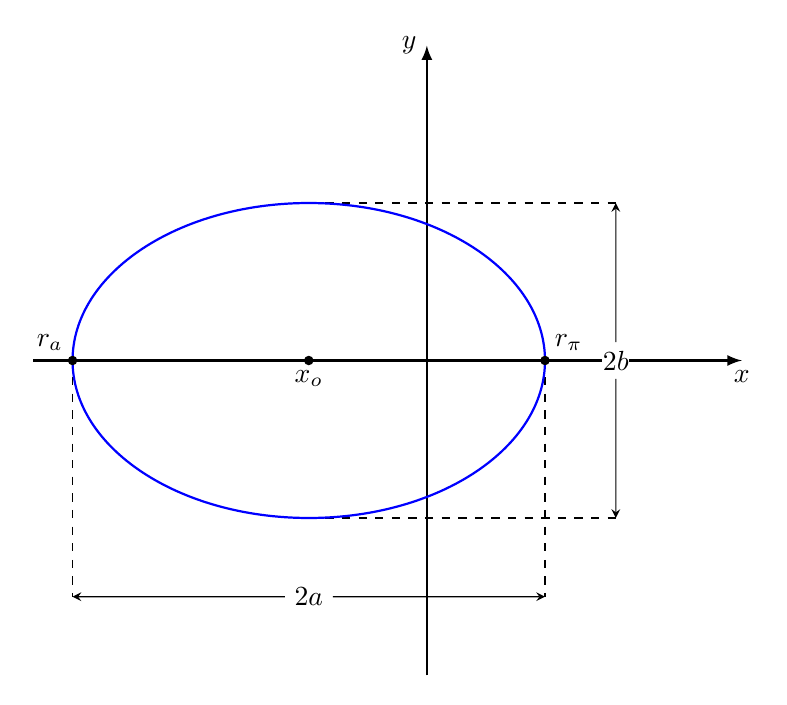
\begin{tikzpicture}
		%Grid
%		\draw[thin, dotted] (0,0) grid (8,8);
%		\foreach \i in {1,...,8}
%		{
%			\node at (\i,-2ex) {\i};	
%		}
%		\foreach \i in {1,...,8}
%		{
%			\node at (-2ex,\i) {\i};	
%		}
%		\node at (-2ex,-2ex) {0};
		
		% Axis
		\draw[-latex, thick] (5,0) -- (5,8) node[left] {$y$};
		\draw[-latex, thick] (0,4) -- (9,4) node[below] {$x$};
		
		% Lines
		\draw[dashed] (0.5,4) -- (0.5,1);
		\draw[dashed] (6.5,4) -- (6.5,1);
		%
		\draw[dashed] (3.5,2) -- (7.4,2);
		\draw[dashed] (3.5,6) -- (7.4,6);
		%% Labeled
		\midlinelabel{0.5,1}{6.5,1}{$2a$}
		%
		\midlinelabell{7.4,2}{7.4,6}{$2b$}
		
		% Ellipse
		\draw[blue, thick] (3.5,4) circle [x radius = 3, y radius = 2];
		
		% Points
		\draw[fill=black] (3.5,4) circle [radius=1.5pt] node[below] {$x_o$};
		\draw[fill=black] (0.5,4) circle [radius=1.5pt] node[above left] {$r_a$};
		\draw[fill=black] (6.5,4) circle [radius=1.5pt] node[above right] {$r_\pi$};
	\end{tikzpicture}
	
\end{document}